%https://physagreg.fr/schemas-figures-physique-svg-tikz.php
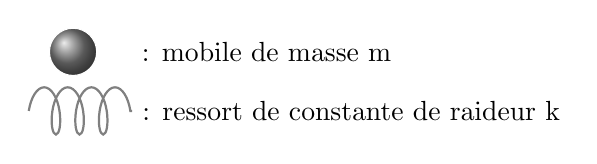
\begin{tikzpicture} [scale=0.75, decoration={coil,aspect=0.4,segment length=3mm,amplitude=3mm}]
%decoration : gère l'aspect du ressort par l'instruction decorate
\tikzset{ressort/.style={thick,gray,smooth}} %définition d'un style de ressort

\begin{scope}
\draw [rounded corners=4pt,color=white,ball color=gray,smooth] (0,-2.5) circle (0.4) node [right=0.75cm,black] {: mobile de masse m} ;
\draw[ressort,decorate,rotate=0] (-0.75,-3.5)--(1,-3.5) node [right=0cm,black] {: ressort de constante de raideur k};
\end{scope}
\end{tikzpicture} 
